\section{Shared Broadcast and Multicast Tree problem}
\label{sec:SBT}

A feasible solution to an SMT instance is a Steiner tree spanning a set $D$ of destinations in $G$.
ssume the tree $T=(V_T, E_T)$ depicted in Fig. \ref{fig:objexp} to be one such solution.
Any node $s\in D$ can initiate a transmission, and all the remaining destinations must receive it.
Consider the node $i$ with three neighbours $i_1$, $i_2$ and $i_3$ ordered by decreasing distance from $i$.
If the transmitting node is $a$, $b$ or $i_1$, then the signal reaches $i$ via arc $(i_1,i)$ and all nodes in the subtree $T_{i_1/i}$ highlighted by the grey area have already received the signal, and so $i$ does not have to send it back to $i_1$.
It suffices that $i$ forwards the signal to its most distant neighbour except from $i_1$, which is $i_2$.
By using the power level $p_{ii_2}$ and due to the wireless advantage, the message reaches all the neighbours that have not received it yet.
On the other hand, if the transmission is initiated by a destination from $T\setminus T_{i_1/i}$ (outside the grey area), then $i$ has to forward it to its most distant neighbour $i_1$, from where it will be relayed to all nodes that have not received the signal.
%
\begin{figure}[h!]
	\centering
	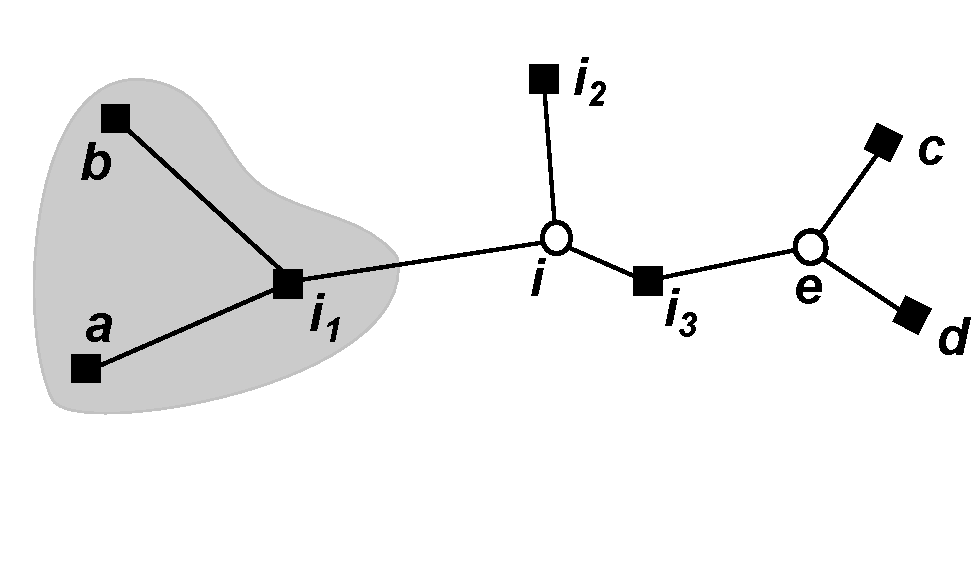
\includegraphics[height=1.6in]{objexp}
	\caption{A simple feasible solution illustrating the calculation of a contribution of node $i$ to the objective function.
		 Destinations and Steiner nodes are denoted by solid squares and empty circles, respectively.}
	\label{fig:objexp}
\end{figure}
%
The objective function captures the entire network structure, and takes account of the  frequency of usage of certain power levels.
In the example above, node $i$ uses power level $p_{ii_2}$ every time source of the relayed signal lies in the subtree $T_{i_1/i}$ which contains three potential sources.
The power level $p_{ii_1}$ is used  whenever the source lies outside of $T_{i_1/i}$, which applies to four sources.
The contribution of node $i$ to the objective function is thus $3p_{ii_2} + 4p_{ii_1}$.
The total cost of $T$ is the sum over all nodes' contributions.
In general, the total power consumption, or cost, is
$$
c(T) = \sum\limits_{i\in V_T}\left[\text{nod}(T_{i_1/i})p_{ii_2} + \text{nod}(T\setminus T_{i_1/i})p_{ii_1}\right].
$$ 
\begin{problem}
\label{def:problem}
(SMT): Find a Steiner tree $T$ of $(G,D)$ minimizing $c(T)$.
\end{problem}
Like most of the wireless network design problems presented in the literature, SMT is NP-hard. This follows from the NP-hardness of SBT\cite{Papadimitriou06SBT}, which is the special case of Problem \ref{def:problem} where $D=V$.
